\documentclass[tikz,border=5pt]{standalone}
\usepackage{times}
\usepackage{amsmath}
\usetikzlibrary{arrows.meta,decorations.pathreplacing}
\begin{document}
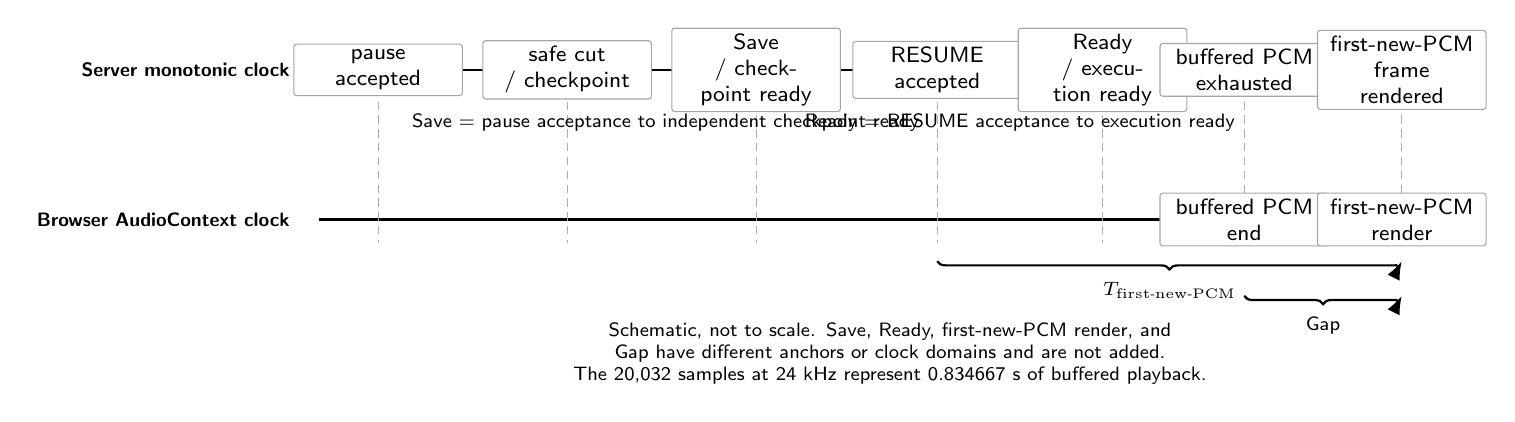
\begin{tikzpicture}[
  font=\sffamily\footnotesize,
  >=Latex,
  event/.style={fill=white,draw=black!35,rounded corners=1pt,
                align=center,inner sep=2pt,text width=2.0cm},
  lane/.style={->,thick},
  metric/.style={decorate,decoration={brace,amplitude=3pt,mirror},
                 thick,->},
  note/.style={align=center,font=\sffamily\scriptsize}
]
\node[anchor=east,font=\sffamily\scriptsize\bfseries] at (0,1.15)
  {Server monotonic clock};
\node[anchor=east,font=\sffamily\scriptsize\bfseries] at (0,-0.75)
  {Browser AudioContext clock};
\draw[lane] (0.25,1.15) -- (14.8,1.15);
\draw[lane] (0.25,-0.75) -- (14.8,-0.75);

\foreach \x/\eventlabel in {
  1.0/{pause\\accepted},
  3.4/{safe cut\\/ checkpoint},
  5.8/{Save\\/ checkpoint ready},
  8.1/{RESUME\\accepted},
  10.2/{Ready\\/ execution ready},
  12.0/{buffered PCM\\exhausted},
  14.0/{first-new-PCM\\frame\\rendered}}
  {
    \draw[densely dashed,gray!65] (\x,1.45) -- (\x,-1.05);
    \node[event] at (\x,1.15) {\eventlabel};
  }
\node[event] at (12.0,-0.75) {buffered PCM\\end};
\node[event] at (14.0,-0.75) {first-new-PCM\\render};
\node[note] at (4.65,0.48) {Save = pause acceptance to independent checkpoint ready};
\node[note] at (9.15,0.48) {Ready = RESUME acceptance to execution ready};
\draw[metric] (8.1,-1.28) -- node[below=4pt,note]
  {$T_{\mathrm{first\text{-}new\text{-}PCM}}$}
  (14.0,-1.28);
\draw[metric] (12.0,-1.72) -- node[below=4pt,note]
  {Gap}
  (14.0,-1.72);
\node[note,text width=11.5cm] at (7.5,-2.45)
  {Schematic, not to scale. Save, Ready, first-new-PCM render, and Gap
   have different anchors or clock domains and are not added.\\
   The 20,032 samples at 24 kHz represent 0.834667 s of buffered playback.};
\end{tikzpicture}
\end{document}
